MSFvenom\cite{msfvenom} herramienta que pertenece al framework de \textit{Metasploit}\cite{metasploit} (figura \ref{fig:logo-metasploit}). \textit{MSFvenom} es la combinación de otras dos herramientas, \textit{MSFpayload} y \textit{MSFencode}. \textit{MSFpayload} se encarga de generar payloads para distintas plataformas, mientras que \textit{MSFencode} se encarga de codificar dichos payloads con el objetivo de evadir la detección mediante el uso de antivirus. \textit{MSFvenom} reemplazó a estas dos herramientas el 18 de junio de 2015.\\

\begin{figure}[h]
    \centering
    
\includegraphics[width=0.20\textwidth]{images/sections/tools/metasploit-logo.png}
    \caption{Logo de \textit{Metasploit}}
    \label{fig:logo-metasploit}
\end{figure}

Las ventajas de \textit{MSFvenom} son:
\begin{itemize}
    \item Se simplifica la generación de payloads y los intentos de codificación de éstos.
    \item Se presenta como una herramienta estándar que ayuda a los auditores y a cualquier usuario su manejo. Es realmente intuitiva y con fácil aprendizaje.
    \item El rendimiento ha sido mejorado considerablemente.
\end{itemize}

\textit{MSFvenom} dispone de una amplia gama de opciones (figura \ref{fig:ayuda-msfvenom}):

\begin{figure}[h]
    \centering
    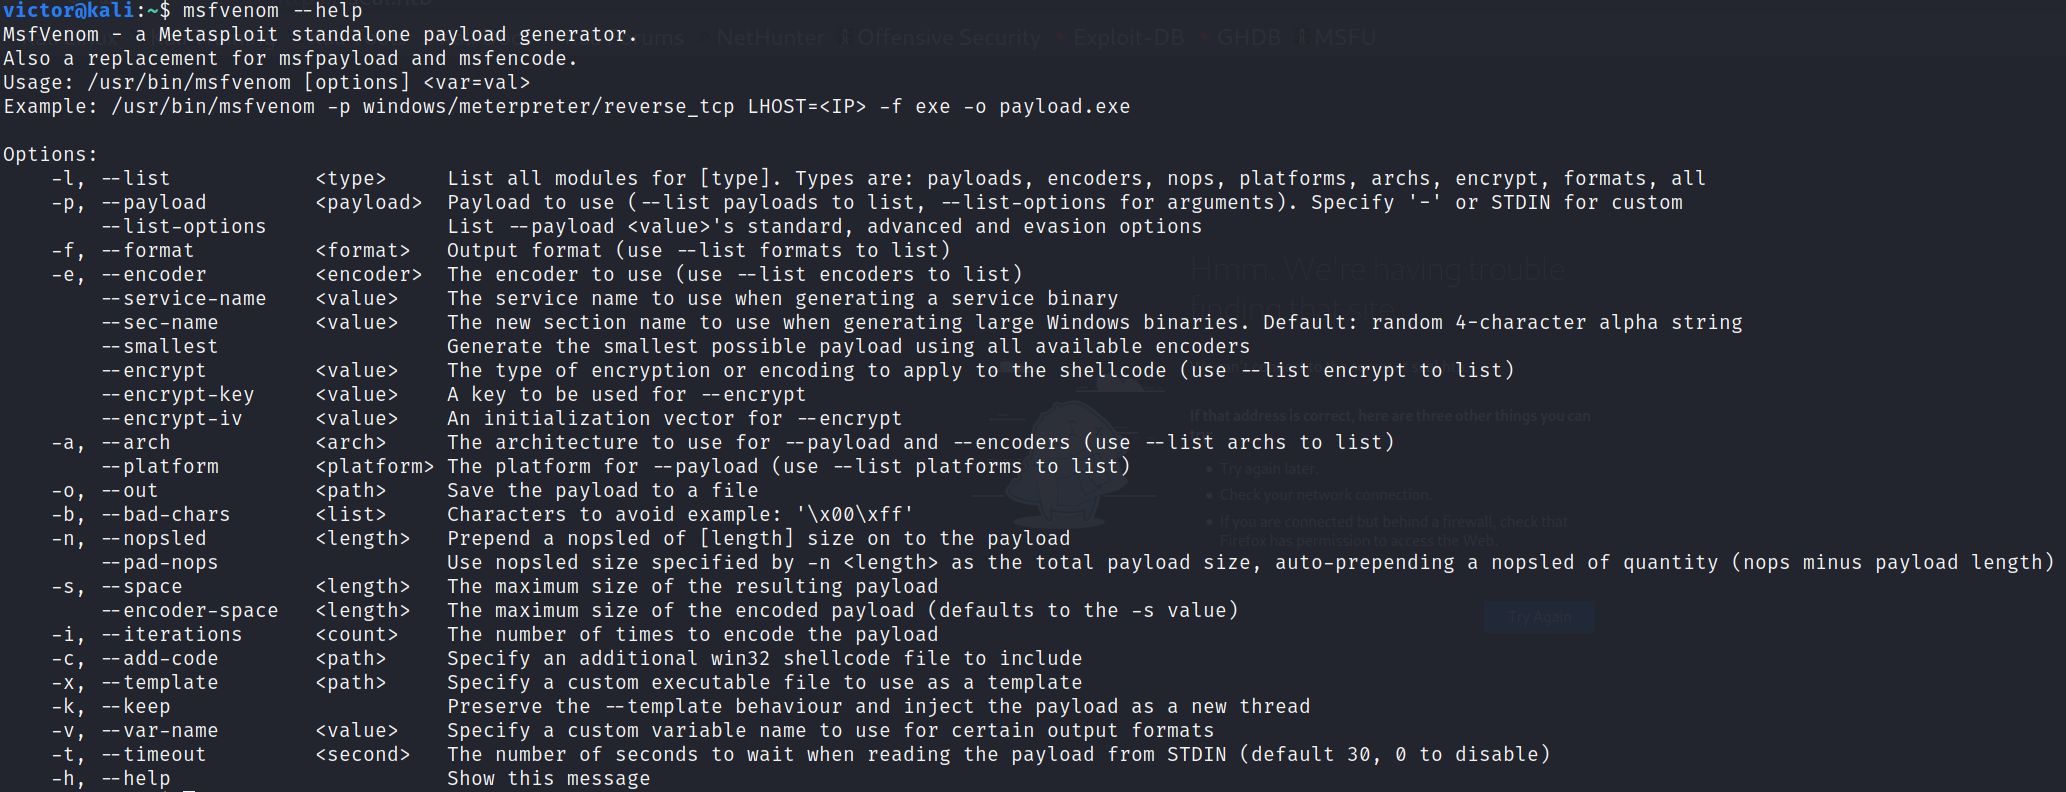
\includegraphics[width=1.0\textwidth]{images/sections/tools/msfvenom-help.png}
    \caption{Ayuda de \textit{MSFvenom}}
    \label{fig:ayuda-msfvenom}
\end{figure}